\section{Introduction}
\label{sec:introduction}

\begin{figure*}[t]
\vspace{-0.75em}
  \centering
  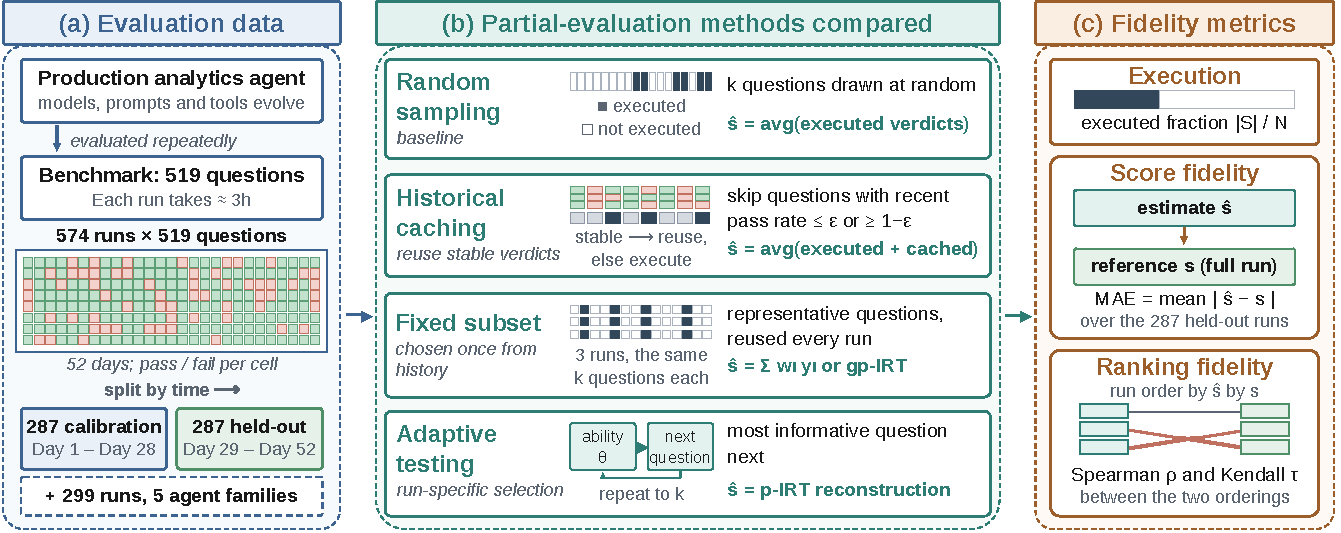
\includegraphics[width=0.9\textwidth]{figures/experiment_overview_v6.2.pdf}
  \caption{Overview of the study. \textbf{(a)} Historical evaluation runs of a
  production analytics agent, split by time into calibration and held-out test
  runs. \textbf{(b)} The four partial-evaluation methods compared: each executes
  a subset $S\subseteq\mathcal{Q}$ and reports an estimate $\hat{s}$ of the pass
  rate $s$ of a complete run. \textbf{(c)} Test on the 287 held-out runs:
  pass-rate MAE against the complete run (lower is better) and Spearman and
  Kendall rank correlation (higher is better).}
  \vspace{-0.75em}
  \label{fig:overview}
\end{figure*}


Production LLM agents require repeated evaluation as their models, prompts,
tools, and surrounding systems evolve. Each benchmark item may involve a
multi-step trajectory with repeated model calls, tool use, stateful interaction,
and task-specific grading; stochasticity may also require repeated trials
\citep{kapoor2026holistic,yao2024tau,jimenez2024swe}. 
Our work is motivated by this challenge in the development of a deployed analytics agent, which serves 
tens of thousands of monthly active users.
Its development and monitoring generate tens of thousands of evaluation runs.
Benchmark evaluation is a major component of this workload. Each run of a central 519-question benchmark 
takes approximately three hours. This
makes cost- and time-efficient
measurement important for continuous development.


Prior work reduces LLM evaluation cost through subset selection,
score reconstruction, and adaptive testing
\citep{vivek2024anchor,maiapolo2024tinybenchmarks,perlitz2024efficient,kipnis2025metabench,yuan2025beyond,truong2025reliable}. These methods are primarily calibrated on
responses of distinct models evaluated on public benchmarks.
Less is known about recurring evaluation of an evolving production agent, where
temporally ordered outcomes from earlier runs can inform later
evaluations.

We therefore ask how faithfully partial evaluation can stand in for the complete
benchmark throughout continuous agent development, along two axes:
\textbf{score fidelity}, the tradeoff between the number of questions executed and error
in the estimated full-benchmark score, and \textbf{ranking fidelity}, how
well rankings among evaluation runs are preserved by each method.


We compare random sampling with three uses of historical evaluation data:
caching reuses stable outcomes, fixed subsets execute representative
questions, and adaptive testing selects each next question based on responses in the current run \citep{maiapolo2024tinybenchmarks,truong2025reliable}. 
We use real historical data from our production agent: 574 benchmark runs collected over 52
days, split into 287 calibration and 287 held-out test runs (Fig.~\ref{fig:overview}).


Our results show that partial evaluation can closely recover full-benchmark
performance with substantially fewer executions. 
Multidimensional 2PL adaptive testing provides the strongest score fidelity:
executing 200 of 519 questions (38.5\% of a complete run) yields 1.03
percentage points (pp) of pass-rate MAE. 
Partial evaluation also
preserves rankings: at 300 questions, the best adaptive configuration reaches
0.992 Spearman correlation with full-benchmark rankings. Difficulty-stratified
fixed subsets give the strongest non-adaptive results, and we deployed them for
their operational simplicity. We further validate this choice through cross-agent transfer and calibration-window sensitivity. 


Our contributions are as follows:\vspace{-0.5em}

\begin{itemize}\itemsep -0.3em
  \item We study recurring evaluation of an evolving production agent using 574
        historical benchmark runs and a temporally held-out protocol.
  \item We compare the score- and ranking-fidelity tradeoffs of random sampling,
        historical caching, fixed subsets, and adaptive testing.
  \item We analyze method design choices and validate difficulty-stratified
        fixed subsets through transfer to five agent families and sensitivity
        to calibration history.
  \item We derive practical recommendations from these results and our
        deployment experience in a production evaluation workflow.
\end{itemize}

